\chapter{Teaching Your PI Controller to Behave (Part VIII)}

We are now on the eight part of a ten part series about teaching your PI controller to behave like you want it to.  At the heart of this discussion is a proposed tuning technique which allows you to be more proactive with the tuning process and reduce the amount of empirical guesswork at the back-end of your design process.  TI has already used this tuning technique on several motor control designs with good success!  But as with any “parameter based” design process, the results are only as good as how well you know your parameters.  In summary, for a permanent magnet synchronous machine, we need to know the following parameters to tune the PI loops:
\begin{itemize}
    \item $R_s$ (motor stator resistance)
    \item $L_s$ (motor stator inductance)
    \item $P$ (\# of motor poles)
    \item $\lambda_r$ (rotor flux)
    \item $J$ (system inertia)
\end{itemize}

If you’re lucky, the motor data sheet may have some of this information.  But in many cases you’re on your own trying to figure out what they are.  But don’t despair!  TI has just released a new sensorless Field Oriented Control algorithm called InstaSPIN-FOC which can measure most of these parameters for you automatically!  Figure \ref{fig:08_01} is a high level diagram of InstaSPIN-FOC, which shows its three distinct components:

\begin{enumerate}
    \item Motor ID:  This algorithm interrogates the motor to gather most of the parameters above.  It is usually run just once during the commissioning process for a particular motor.
    \item FAST:  This is the observer which calculates the real-time motor parameters needed for Field Oriented Control.  The neat part is that it doesn’t require a shaft angle or speed sensor to do it!  F.A.S.T. stands for Flux, Angle, Speed and Torque, which represent the main outputs of the FAST observer.  A diagram of how the FAST observer can be used in a Field Oriented Controller is shown in figure \ref{fig:08_02}.
    \item PowerWarp:  This is a special energy savings operating mode used to reduce the copper losses in AC Induction Machines, especially during light-load conditions.
\end{enumerate}
\begin{figure}[H]
    \centering
    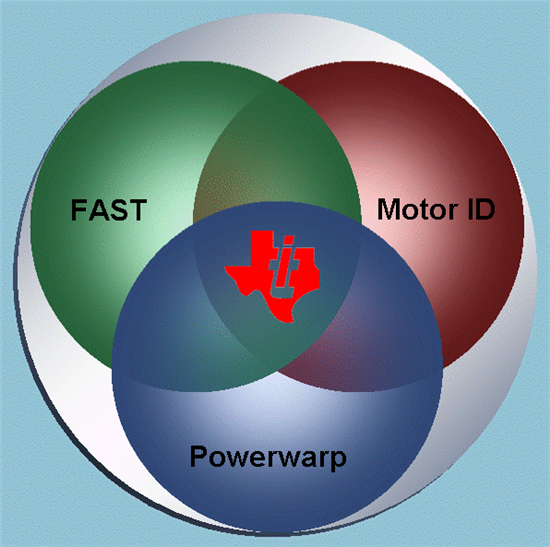
\includegraphics[width=0.8\linewidth]{08/01}
    \caption{Components of InstaSPIN-FOC}
    \label{fig:08_01}
\end{figure}

There is actually a fourth component of InstaSPIN-FOC which is part of the motor ID function, and runs in real time to provide continuous estimates of the stator resistance.  This is the parameter that typically changes the most as the motor heats up during operation.  Monitoring it in real time significantly improves the performance of the FAST observer, and also allows you to dynamically change $K_b$ in the current PI controllers to maintain pole/zero cancellation.  I have a lot more to say about this feature, as well as the other components of InstaSPIN-FOC in an upcoming blog series.

\begin{figure}[H]
    \centering
    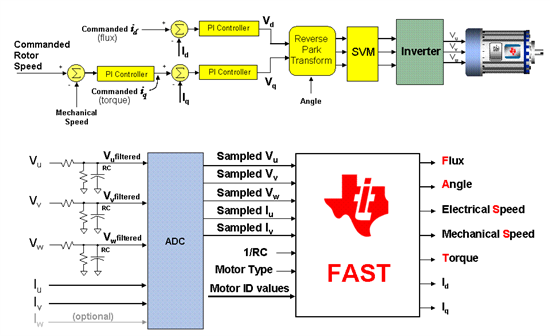
\includegraphics[width=0.8\linewidth]{08/02}
    \caption{ FAST Embedded in a Field Oriented Controller}
    \label{fig:08_02}
\end{figure}

So we see that InstaSPIN-FOC provides measurements for $R_s$, $L_s$, and the rotor flux.  Fortunately, the number of motor poles is often listed on most data sheets, or can easily be determined empirically.  This leaves only system inertia ($J$) that is unknown.  But the entire velocity loop tuning procedure hangs on whether we accurately know what this parameter is.  Even though InstaSPIN-FOC doesn’t directly measure inertia for you, the following is a proposed procedure for how to use the outputs from FAST to measure inertia:

\begin{enumerate}
\item Design the current controller by setting $K_a = L_s/\tau$, or $\pi L_s/(10T_s)$, whichever is lower.  Recall that $\tau$ equals the velocity feedback filter time constant, $L_s$ = the stator winding inductance, and $T_s$ = sampling period.  Also set $K_b = R_s/L_s$.

\item Disable the velocity loop and use only the current loop.  Set $I_d =0$, and apply a fixed value of q-axis current which is sufficient to cause the motor and load to accelerate through a good portion of the rated speed range.

\item \label{step:08_03} As the motor is ramping up to speed, periodically sample and record the values for motor mechanical speed ($\omega(n)$ in \unit{\radian\per\second}) and also the motor torque ($T_1(n)$ in \unit{\newton\meter}).  Both of these measurements are outputs from the FAST observer.  The motor torque should be pretty consistent since $I_q$ is constant, and the motor speed should monotonically increase for a well behaved load.  For example, figure \ref{fig:08_03} shows the simulated samples of the speed output from the FAST observer for a permanent magnet motor driving a fan load with fixed inertia.  The sampling frequency is \qty{200}{\milli\second} over a \qty{4}{\second} span, resulting in a total of 20 samples.
% Note: here I found the first typo in those blogposts: it said 200 mS vs 200 ms
\item Now enable the velocity loop and set the PI coefficients to very low values that will barely allow you to spin the motor up to speed.  Since we don’t know inertia yet, we can’t accurately specify the velocity loop coefficients anyway.  Don’t worry about the dynamic response of the system at this point, since we are only interested in steady state performance.

\item Command the motor to go to each of the recorded speeds from step \ref{step:08_03} by monitoring the speed output of the FAST observer.  After the system response has completely settled out for each commanded velocity, again record the torque values from FAST ($T_2(n)$ in \unit{\newton\meter}).  This torque will correspond to the static load torque apart from any acceleration artifacts.

\item We now have all the data required to solve for inertia as a function of time ($J(n)$ in \unit{\kg\m\squared}) by using the following difference equation:
\begin{equation}\label{eq:8_1}
    \hat J(n) = \frac{2 T_s \left(T_1(n-1) - T_2 (n-1)\right)}{\omega(n)-\omega(n-2)}
\end{equation}
where
\begin{itemize}
    \item $J(n)$ is the inertia at sample time "$n$" (\unit{\kg\m\squared})

    \item $T_s$ is the periodic sampling period (\unit{s})

    \item $T_1$ is the total torque consisting of static friction and acceleration torque (\unit{\newton\meter}) from the FAST observer

    \item $T_2$ is the static friction torque only (\unit{\newton\meter}) from the FAST observer

    \item $w$ is the mechanical speed measurement (\unit{\radian\per\second}) from the FAST observer
\end{itemize}
\end{enumerate}

\begin{figure}[H]
    \centering
    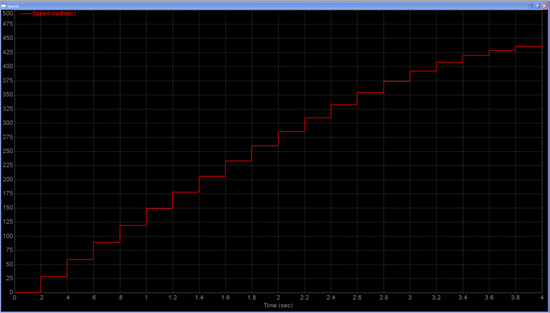
\includegraphics[width=0.8\linewidth]{08/03}
    \caption{Simulated Speed Samples of a Fan Controller with Fixed Inertia}
    \label{fig:08_03}
\end{figure}


Figure \ref{fig:08_04} shows an example inertia plot using \ref{eq:8_1} applied to the data from figure \ref{fig:08_03}.  The estimated values are plotted in red at each time step along with the actual load inertia in green.  In this particular scenario, the inertia is constant and the torque ripple is zero, making it the best condition to estimate inertia.  As you can see, the results are most accurate for the range in figure \ref{fig:08_03} where the acceleration is fairly constant.  In this case you would simply time-average those inertia estimates to come up with a single value for system inertia.  But what if you have excessive torque ripple, such as a compressor load?  In that case, you can think of the torque ripple as unwanted noise in the system.  To maximize the signal-to-noise ratio, you should set the q-axis current as high as possible to increase the ratio between the $T_1$ and $T_2$ torque readings.  It would also help to do a time average of the steady-state torque readings at each velocity point.



\begin{figure}[H]
    \centering
    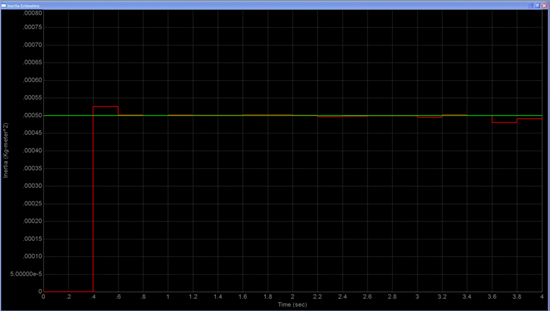
\includegraphics[width=0.8\linewidth]{08/04}
    \caption{Estimated vs. Actual Values of System Inertia as a Function of Time}
    \label{fig:08_04}
\end{figure}

For applications where inertia is a function of velocity (like a centrifuge load), this technique can provide a distinct advantage over other techniques.  Since equation \ref{eq:8_1} calculates inertia as a function of time, and you also have data for motor speed as a function of time from step \ref{step:08_03}, you can combine the two sets of data to correlate inertia as a function of speed.  Having this data in a Look Up Table in memory allows you to dynamically update the $K_c$ term in the velocity PI controller as the speed changes to optimize the response at any speed.

So far, we have discussed PI tuning in generic terms which are mostly independent of the control topology.  In my next blog, I want to focus specifically on some of the more subtle points to consider when designing PI controllers for Field Oriented Control systems.  Until then\dots

\;\\\;\\
Keep Those Motors Spinning,\\

\includegraphics[width=0.2\linewidth]{01/04_dave}
\vfill
\textit{Apr 14 2013 22:35 PM}